\section{Related Work}
Adjusted MAT structure for only printing the outer wall, rest area to be filled using normal infill. \cite{Moesen2011}
\Cref{moessen}

Figuring out underfilling and overfilling arteas in concentric fill and using single squigly lines to prevent overfilling. \cite{Jin2017}
\Cref{jin}

Using variable width lines to fit a precise amount of lines using the MAT.
\cite{Ding2016a} apply the method from \cite{kao1998optimal}.
\Cref{ding}

\begin{figure}
\begin{subfigure}{0.45\columnwidth}
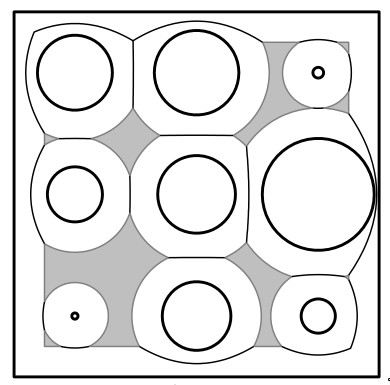
\includegraphics[width=\columnwidth]{sources/related_work/moessen.jpg}
\caption{asfd}
\label{moessen}
\end{subfigure}
\begin{subfigure}{0.45\columnwidth}
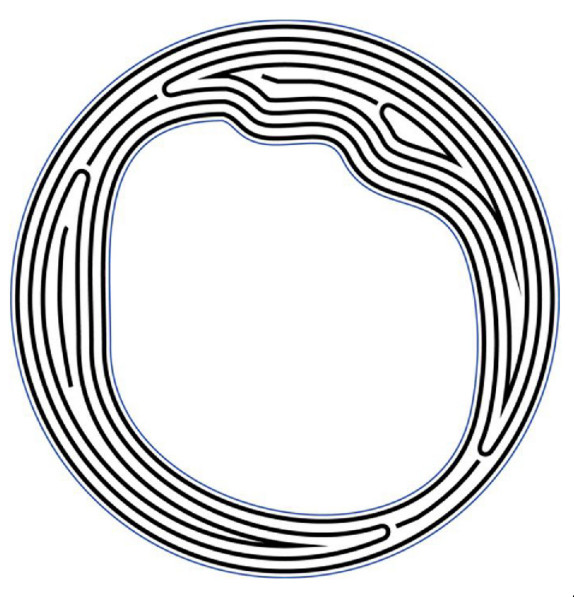
\includegraphics[width=\columnwidth]{sources/related_work/jin.jpg}
\caption{asfd}
\label{jin}
\end{subfigure}
\end{figure}

\begin{figure}
\centering
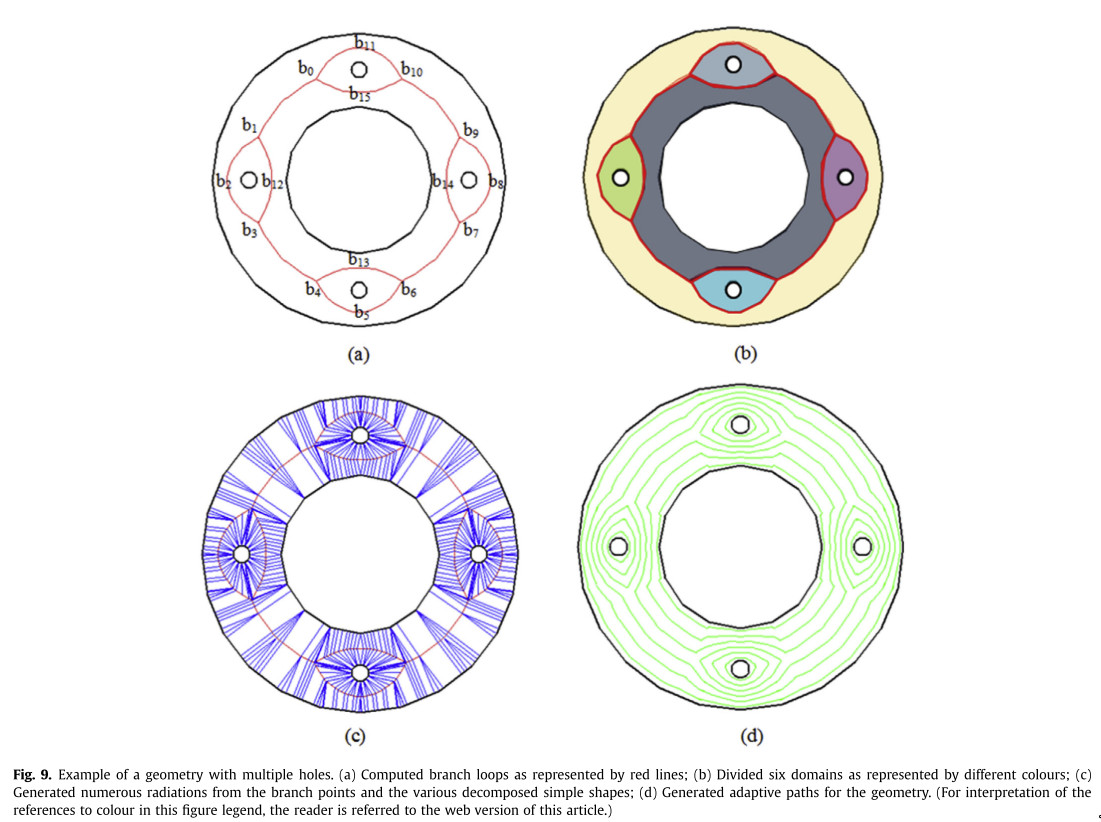
\includegraphics[width=\columnwidth]{sources/related_work/ding.jpg}
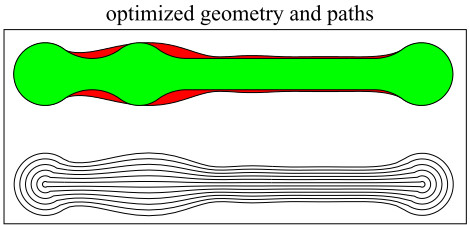
\includegraphics[width=.7\columnwidth]{sources/related_work/kao.jpg}
\caption{Path planning strategies proposed by Kao (bottom) and employed in FDM by Ding et al (top).}
\label{ding}
\end{figure}